\documentclass[tikz,border=10pt]{standalone}
\usepackage[T1]{fontenc}
\usepackage{lmodern}
\usepackage{tikz}
\usetikzlibrary{arrows.meta,calc,decorations.pathreplacing,fit,matrix,positioning}

\definecolor{cornellred}{HTML}{B31B1B}
\definecolor{ink}{HTML}{202124}
\definecolor{muted}{HTML}{667085}
\definecolor{line}{HTML}{AEB8C6}
\definecolor{paper}{HTML}{FFFFFF}
\definecolor{soft}{HTML}{F5F7FA}
\definecolor{camera}{HTML}{E8F4FF}
\definecolor{memory}{HTML}{F0F7EC}
\definecolor{compute}{HTML}{FFF3E6}
\definecolor{display}{HTML}{F7ECF3}
\definecolor{verify}{HTML}{EFEAFE}

\tikzset{
  font=\sffamily,
  flow/.style={
    -{Latex[length=2.6mm,width=1.8mm]},
    draw=muted,
    line width=0.8pt,
    rounded corners=2pt
  },
  dataflow/.style={
    flow,
    draw=cornellred
  },
  block/.style={
    rectangle,
    rounded corners=3pt,
    draw=line,
    line width=0.8pt,
    fill=paper,
    align=center,
    minimum width=28mm,
    minimum height=10mm,
    inner xsep=4pt,
    inner ysep=4pt
  },
  smallblock/.style={
    block,
    minimum width=22mm,
    minimum height=8mm,
    font=\sffamily\scriptsize
  },
  title/.style={
    font=\sffamily\bfseries\large,
    text=ink
  },
  labeltext/.style={
    font=\sffamily\scriptsize,
    text=muted,
    align=center
  },
  camera_block/.style={block, fill=camera, draw=blue!45!black},
  memory_block/.style={block, fill=memory, draw=green!45!black},
  compute_block/.style={block, fill=compute, draw=orange!65!black},
  display_block/.style={block, fill=display, draw=purple!45!black},
  verify_block/.style={block, fill=verify, draw=violet!50!black},
  groupbox/.style={
    draw=line,
    rounded corners=5pt,
    line width=0.7pt,
    fill=soft,
    inner sep=7pt
  }
}


\usetikzlibrary{arrows.meta,positioning,fit,calc}

\begin{document}
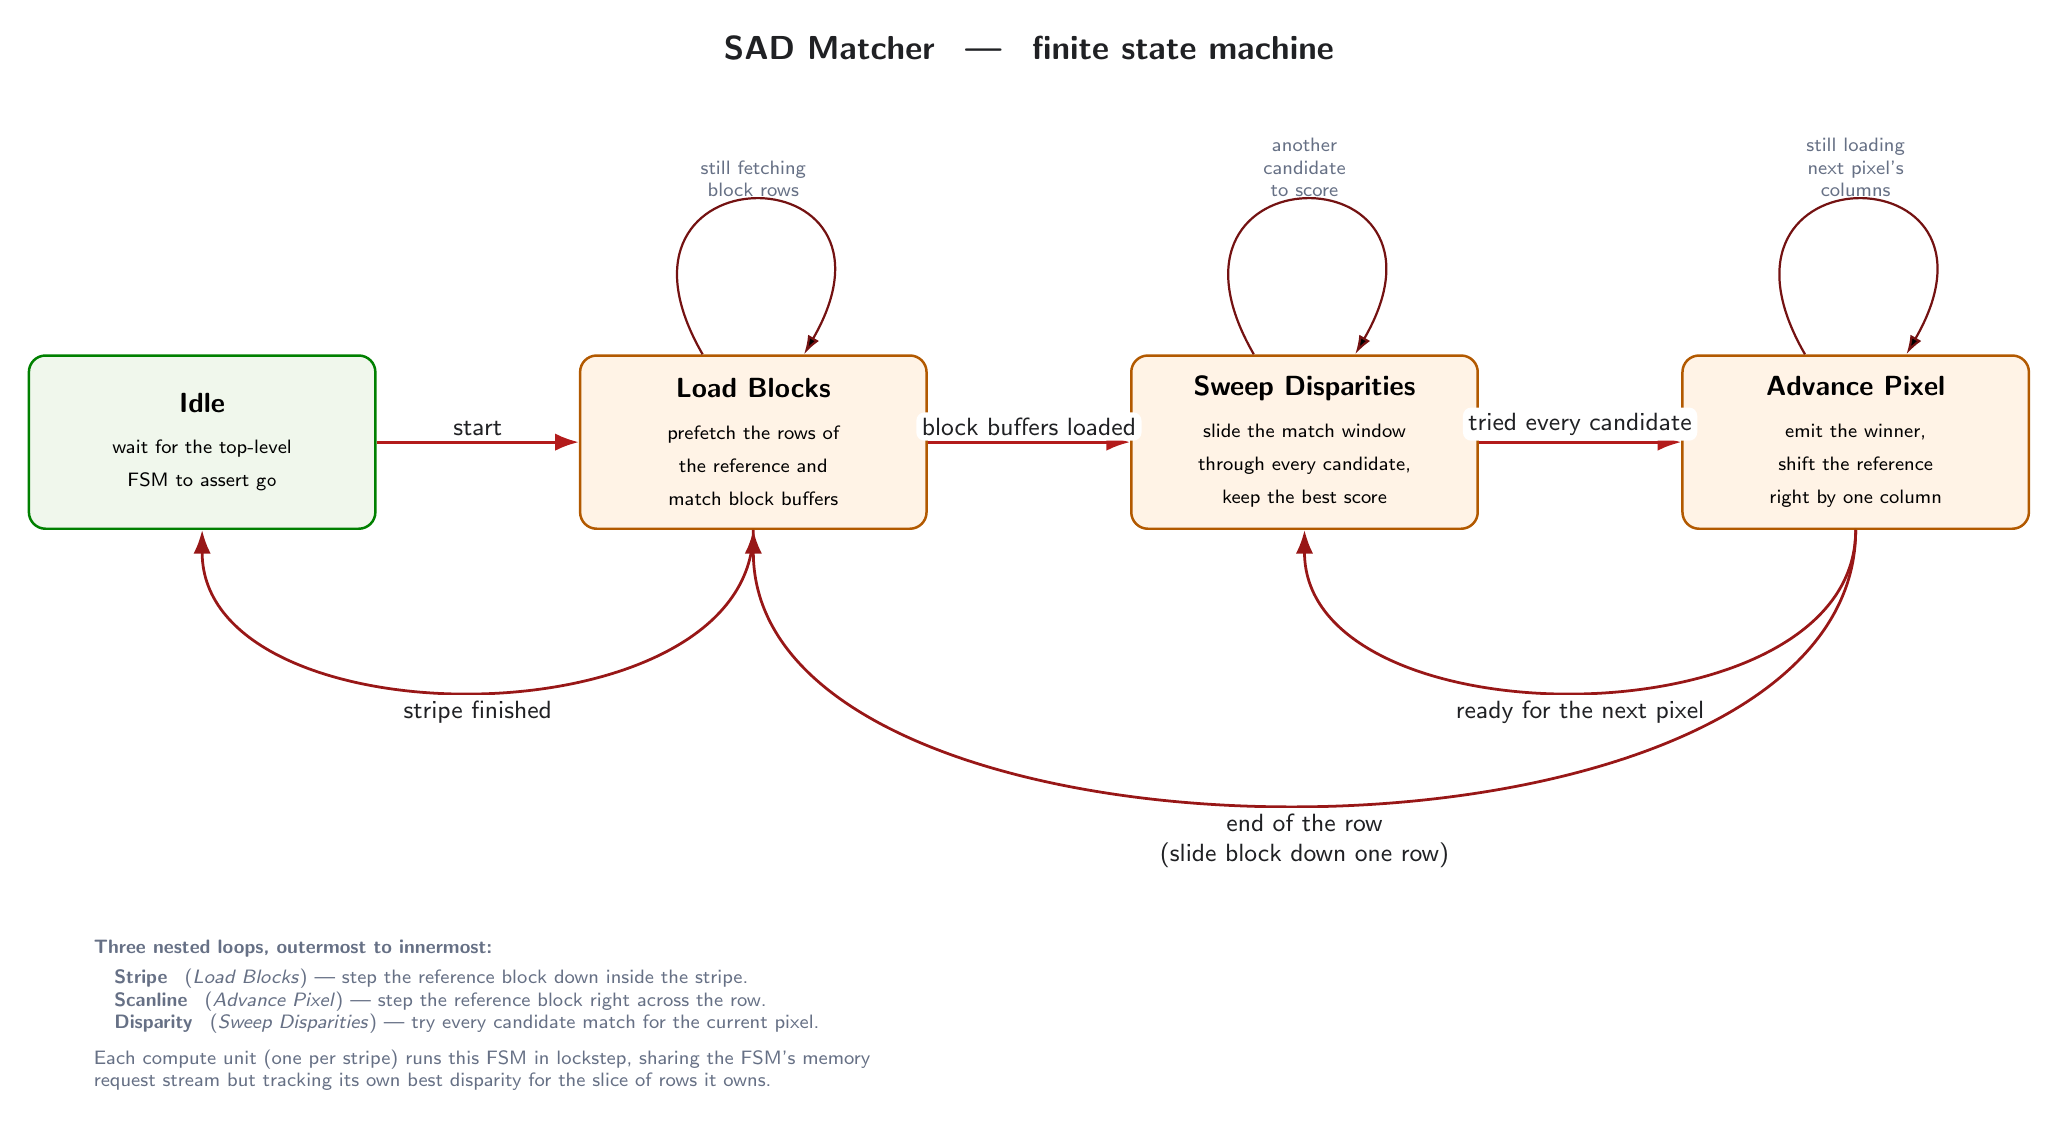
\begin{tikzpicture}[
  font=\sffamily,
  %===========================================================
  % State node styles
  %===========================================================
  state/.style={
    rectangle,
    rounded corners=6pt,
    draw=line,
    line width=0.9pt,
    fill=paper,
    align=center,
    minimum width=44mm,
    minimum height=22mm,
    inner xsep=6pt,
    inner ysep=6pt
  },
  state_idle/.style={state, fill=memory,  draw=green!50!black},
  state_busy/.style={state, fill=compute, draw=orange!70!black},
  %===========================================================
  % Transitions
  %===========================================================
  fwd/.style={
    -{Latex[length=3mm,width=2.2mm]},
    draw=cornellred,
    line width=1.0pt,
    rounded corners=3pt
  },
  back/.style={
    -{Latex[length=3mm,width=2.2mm]},
    draw=cornellred!85!black,
    line width=1.0pt
  },
  selfloop/.style={
    -{Latex[length=2.4mm,width=1.6mm]},
    draw=cornellred!65!black,
    line width=0.8pt
  },
  %===========================================================
  % Labels
  %===========================================================
  cond/.style={
    font=\sffamily\small,
    text=ink,
    fill=paper,
    inner sep=2pt,
    align=center
  },
  loopcond/.style={
    font=\sffamily\scriptsize,
    text=muted,
    align=center,
    inner sep=1pt
  }
]
  \node[title] at (0, 5.0) {SAD Matcher \, --- \, finite state machine};

  %====================================================================
  % Four states laid out left-to-right as the forward pipeline.
  % Idle is the entry point; the three busy states form a clockwise
  % loop closed by the back-edges below.
  %====================================================================
  \node[state_idle] (idle)  at (-10.5,  0)
    {\textbf{Idle}\\[3pt]
     \scriptsize{}wait for the top-level\\
     \scriptsize{}FSM to assert \texttt{go}};

  \node[state_busy] (phase) at ( -3.5,  0)
    {\textbf{Load Blocks}\\[3pt]
     \scriptsize{}prefetch the rows of\\
     \scriptsize{}the reference and\\
     \scriptsize{}match block buffers};

  \node[state_busy] (disp)  at (  3.5,  0)
    {\textbf{Sweep Disparities}\\[3pt]
     \scriptsize{}slide the match window\\
     \scriptsize{}through every candidate,\\
     \scriptsize{}keep the best score};

  \node[state_busy] (xinc)  at ( 10.5,  0)
    {\textbf{Advance Pixel}\\[3pt]
     \scriptsize{}emit the winner,\\
     \scriptsize{}shift the reference\\
     \scriptsize{}right by one column};

  %====================================================================
  % Forward path -- along the top, left to right.
  % The labels read like sentences and never mention raw counters.
  %====================================================================
  \draw[fwd] (idle.east)  -- node[cond, above]{start}                 (phase.west);
  \draw[fwd] (phase.east) -- node[cond, above]{block buffers loaded} (disp.west);
  \draw[fwd] (disp.east)  -- node[cond, above]{tried every candidate} (xinc.west);

  %====================================================================
  % Self-loops -- above each busy state.
  % They represent the multi-cycle work the state does internally
  % (waiting on the prefetcher, walking disparity, etc.).
  %====================================================================
  \path[selfloop] (phase) edge[loop above, in=60, out=120, looseness=6, min distance=10mm]
    node[loopcond, above]{still fetching\\block rows} (phase);

  \path[selfloop] (disp)  edge[loop above, in=60, out=120, looseness=6, min distance=10mm]
    node[loopcond, above]{another\\candidate\\to score} (disp);

  \path[selfloop] (xinc)  edge[loop above, in=60, out=120, looseness=6, min distance=10mm]
    node[loopcond, above]{still loading\\next pixel's\\columns} (xinc);

  %====================================================================
  % Back-edges -- below the pipeline.
  %
  %   inner :  Advance Pixel  ->  Sweep Disparities  (next pixel)
  %   outer :  Load Blocks    ->  Idle               (stripe done)
  %      ^- both span the same width and live on opposite sides of the
  %         diagram, so they sit at the same depth without overlapping.
  %
  %   middle:  Advance Pixel  ->  Load Blocks        (end of row)
  %      ^- spans the whole pipeline, so the natural curve goes deeper
  %         and visually wraps the inner and outer arcs.
  %====================================================================
  \draw[back] (xinc.south)  to[out=-90, in=-90, looseness=1.0]
    node[cond, midway, below=1pt]{ready for the next pixel}
    (disp.south);

  \draw[back] (phase.south) to[out=-90, in=-90, looseness=1.0]
    node[cond, midway, below=1pt]{stripe finished}
    (idle.south);

  \draw[back] (xinc.south)  to[out=-90, in=-90, looseness=0.85]
    node[cond, midway, below=1pt]{end of the row\\(slide block down one row)}
    (phase.south);

  %====================================================================
  % Footer / legend
  %====================================================================
  \node[labeltext, align=left, anchor=north west] at (-12, -6.2)
    {\textbf{Three nested loops, outermost to innermost:}\\[3pt]
     \quad \textbf{Stripe}     \, (\textit{Load Blocks})       --- step the reference block down inside the stripe.\\
     \quad \textbf{Scanline}   \, (\textit{Advance Pixel})     --- step the reference block right across the row.\\
     \quad \textbf{Disparity}  \, (\textit{Sweep Disparities}) --- try every candidate match for the current pixel.\\[5pt]
     Each compute unit (one per stripe) runs this FSM in lockstep, sharing the FSM's memory\\
     request stream but tracking its own best disparity for the slice of rows it owns.};

\end{tikzpicture}
\end{document}
